\chapter{Methodology}
% TODO: overview of the chapter


%%%%%%%%%%%%%%%
\section{System architecture}
\label{sec:SystemArchitecture}
As depicted in figure \ref{fig:pa:systemBlockDiagram}, we use the pose estimates calculated using stereo images and \gls{LiDAR} point clouds as relative measurements. ORB SLAM 2 and LegoLOAM algorithms, respectively, are used for this purpose. Furthermore, \gls{GNSS} measurements and orientation estimated from magnetometer measurements act as positional and rotational absolute measurements to the fusion mechanism. The fusion mechanism is an \gls{ES-EKF} with 16 variables in the state space and 15 variables in the error state space. The output of the system consists of a state vector including position, orientation and velocity of the vehicle relative to a global frame of reference. Estimated covariance of the error is also provided, from which, the 99\% confidence interval ($3\sigma$ bound) can be derived. Output is compared with the ground truth provided with the dataset being used, to calculate the resultant error margins.
\begin{figure}[h]
	\begin{center}
	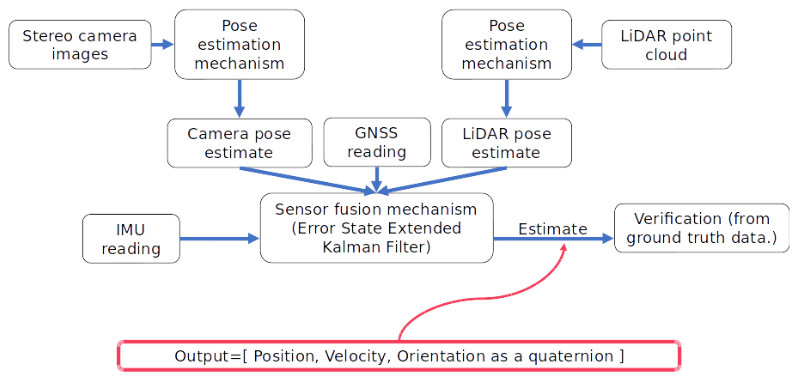
\includegraphics[width=\textwidth]{figs/system-block-diagram.png}
	\end{center}
	\vspace{-0.5cm}
	\caption{System block diagram}
	\label{fig:pa:systemBlockDiagram}
	\vspace{0.5cm}
\end{figure}

The system is implemented on \gls{ROS}, along with evaluation and visualization mechanisms for demonstrating functionality. Main programming language used is Python. Each of the components mentioned in the above discussion will be explained in detail, in the subsequent sections.



%%%%%%%%%%%%%%%
\section{Coordinate frames}
% TODO




%%%%%%%%%%%%%%%
\section{Sensor fusion mechanism}
\subsection{The \gls{ES-EKF}}
As mentioned in section \ref{sec:SystemArchitecture}, the \gls{ES-EKF} currently has 16 state space variables and 15 error state space variables, grouped into 5 sub-vectors, as listed below;
\begin{align}
    \text{State vector: }\textbf{x} &= \left[\begin{matrix}{}\textbf{p}\\\textbf{v}\\\textbf{q}\\\boldsymbol{a_b}\\\boldsymbol{\omega_b}\end{matrix}\right]
\end{align}
where
\begin{align}
    \textbf{p} &= (p_x, p_y, p_z) \text{ position relative to the inertial frame} \nonumber \\
    \textbf{v} &= (v_x, v_y, v_z) \text{ velocity relative to the inertial frame} \nonumber \\
    \textbf{q} &= (q_w, q_x, q_y, q_z) \text{ quaternion relative to the inertial frame} \nonumber \\
    \boldsymbol{a_b} &= (a_{bx}, a_{by}, a_{bz}) \text{ acceleration biases of the IMU relative to the body frame} \nonumber \\
    \boldsymbol{\omega_b} &= (\omega_{bx}, \omega_{by}, \omega_{bz}) \text{ angular velocity biases of the IMU relative to the body frame}
\end{align}
and
\begin{align}
	\text{Error state vector: }\boldsymbol{\delta}\textbf{x} &= \left[\begin{matrix}{}\boldsymbol{\delta}\textbf{p}\\\boldsymbol{\delta}\textbf{v}\\\boldsymbol{\delta}\boldsymbol{\theta}\\\boldsymbol{\delta}\boldsymbol{a_b}\\\boldsymbol{\delta}\boldsymbol{\omega_b}\end{matrix}\right].
\end{align}
Here, $\boldsymbol{\delta}\boldsymbol{\theta}$ is the error in orientation, expressed as an axis-angle vector. Furthermore, $\boldsymbol{\delta}\boldsymbol{a_b}$ and $\boldsymbol{\delta}\boldsymbol{\omega_b}$ are the considered as global errors. The motion model for the prediction step of the filter is given below.\\
State update:
\begin{align}
    \check{\textbf{p}}_k &= \hat{\textbf{p}}_{k-1}+\hat{\textbf{v}}_{k-1}\Delta t + \frac{1}{2} \left( \textbf{R}_{inert,body}\left(\textbf{a}_{m_{k-1}}-\hat{\textbf{a}}_{b_{k-1}}\right)+\textbf{g}\right)\Delta t^2 \\
    \check{\textbf{v}}_k &= \hat{\textbf{v}}_{k-1}+\left(\textbf{R}_{inert,body}\left(\textbf{a}_{m_{k-1}}-\hat{\textbf{a}}_{b_{k-1}}\right)+\textbf{g}\right)\Delta t \\
    \check{\textbf{q}}_k &= \hat{\textbf{q}}_{k-1}\otimes \textbf{q}\left\{\left(\boldsymbol{\omega}_{m_{k-1}}-\hat{\boldsymbol{\omega}}_{b_{k-1}}\right)\Delta t\right\} \\
    \check{\textbf{a}}_{b_k} &= \hat{\textbf{a}}_{b_{k-1}} \\
    \check{\boldsymbol{\omega}}_{b_{k}} &= \hat{\boldsymbol{\omega}}_{b_{k-1}}
\end{align}
with
\begin{align}
	\textbf{a}_{m_{k}} &= \text{Acceleration measured by accelerometer at k\textsuperscript{th} instance}\\
	\boldsymbol{\omega}_{m_{k}} &= \text{Angular velocity measured by gyroscope at k\textsuperscript{th} instance}\\
    \textbf{R}_{inert,body} &= \text{Rotation matrix corresponding to $\hat{\textbf{q}}_{k-1}$} \\
	\textbf{g} &= \text{Gravity vector w.r.t inertial frame}\\
	\otimes &= \text{Quaternion composition operator.}
\end{align}
Covariance matrix update:
\begin{align}
    \Check{\textbf{P}}_k &= \textbf{F}_x\hat{\textbf{P}}_{k-1}\textbf{F}_x^T + \textbf{F}_i\textbf{Q}_i\textbf{F}_i^T
\end{align}
where
\begin{align}
	\textbf{P}_k &= \text{Error state covariance matrix at k\textsuperscript{th} instance}\\
	\textbf{F}_x &= \text{Jacobian of the motion model, relative to the error state, evaluated at zero}\\
	\textbf{F}_i &= \text{Jacobian of the motion model, relative to the process noise,}\nonumber\\
	&\quad\text{evaluated at zero}\\
	\textbf{Q}_i &= \text{Process noise covariance matrix}.
\end{align}
The equations pertaining to the correction process, upon receiving a measurement update is given below.
\begin{align}
    \textbf{K}_k &= \check{\textbf{P}}_k\textbf{H}^T\left(\textbf{H}\check{\textbf{P}}_k\textbf{H}^T+\textbf{V}\right)^{-1} \\
    \hat{\textbf{P}}_k &= \left(\textbf{I}-\textbf{K}_k\textbf{H}\right)\check{\textbf{P}}_k\\
	\hat{\boldsymbol{\delta}\textbf{x}_k} &= \textbf{K}_k \left(\textbf{y}-h\left(\check{\textbf{x}}_k\right)\right).
\end{align}
Here,
\begin{align}
	h(.) &= \text{Measurement function}\\
	\textbf{H} &= \text{Jacobian of the measurement function, relative to the error state,}\nonumber\\
	&\quad\text{ evaluated at zero}\\
	\textbf{V} &= \text{Measurement noise matrix}\\
	\textbf{y} &= \text{Measurement vector}\\
	\textbf{I} &= \text{Identity matrix of suitable dimension}.
\end{align}
For a detailed description of the matrices in above equations, refer Appendix \ref{appendix:ESEKFMatrices}.


\subsection{Stochastic cloning and backward smoothing}
Stochastic cloning 






\begin{table}[h]
\centering
\begin{tabular}{|c | c | c | c|} 
	\hline
	\textbf{Heading1} & \textbf{Heading2} & \textbf{Heading3} & \textbf{Heading4} \\
	\hline
	1 & 6 & 87837 & 787 \\
	\hline
	2 & 7 & 78 & 5415 \\
	\hline
	3 & Banana & 778 & Apple \\
	\hline
\end{tabular}
\caption{Example table}
\label{table:pa:ExampleTable}
\end{table}